\section{Introduction}
\label{sec:introduction}

% Outline: IoT for home entertainment
Internet-of-Things (IoT) technologies are being rapidly adopted in the consumer electronics market.
In addition to their use in traditional home automation systems, IoT technologies have also been applied to home entertainment--for example, with wireless inertial sensors used to track user body movement in sports games. 
Combined with emerging virtual and augmented reality technologies, IoT offers the promise of new immersive and interactive experience for end-users.

Common requirements for such systems include:
\begin{itemize}
\item Integration of heterogeneous devices and services from different vendors;
\item Interactive user experience that emphasize real-time feedback loop;
\item Easy installation and configuration; and
\item Security protection, due to tight integration with the home network.
\end{itemize}

% Outline: existing frameworks and their functionality summary
Many IoT frameworks and ecosystems have been proposed over the last few years to facilitate the development of more sophisticated applications like these.
They typically provide a similar set of framework-level services, including user and device authentication and authorization, device and service discovery, device management, publish-subscribe messaging, and remote access.
Fig.~\ref{fig:service-arch} shows a common hierarchical architecture of IoT services, where ``named entities'' refer to users, devices, and applications that require trust management and utilize rendezvous services to get organized into a coherent home IoT system.

\begin{figure}[!t]
\centering
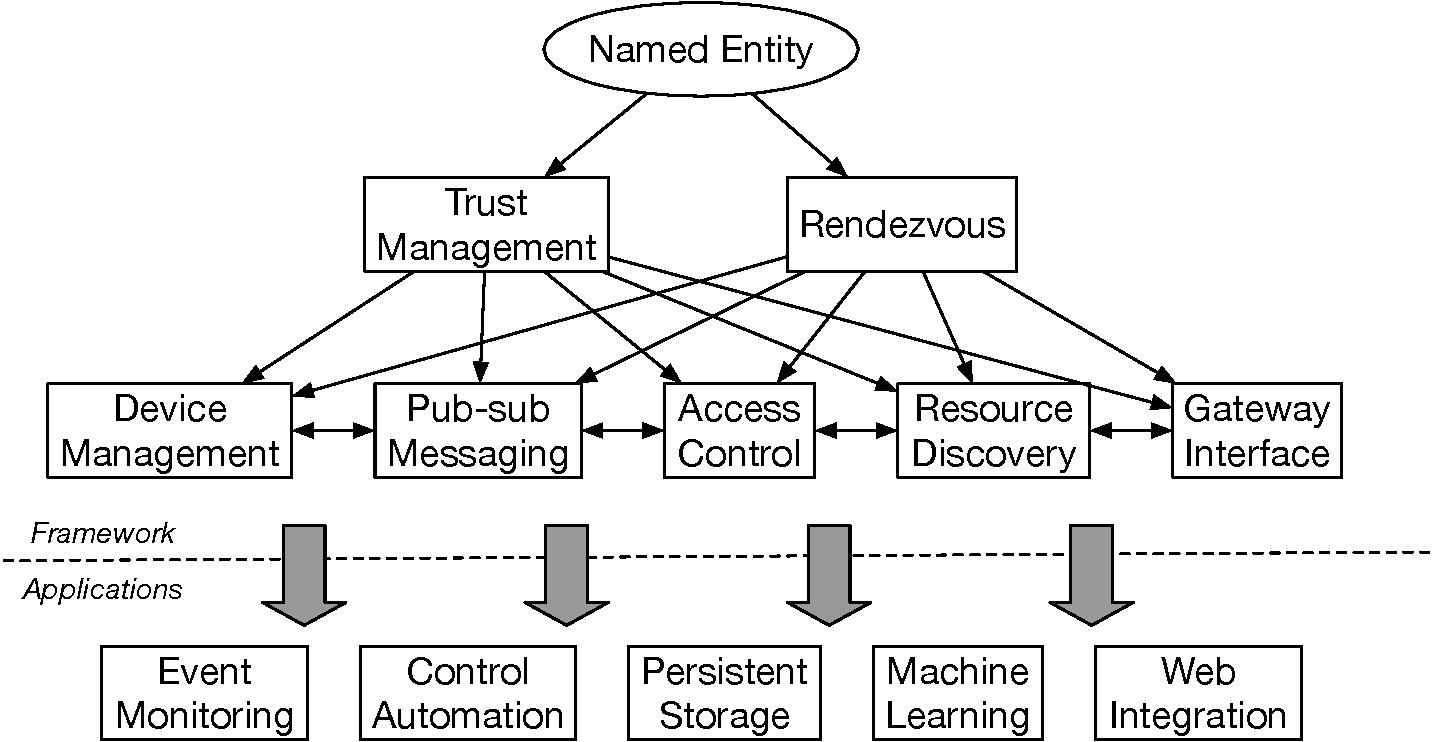
\includegraphics[width=0.95\columnwidth]{service-arch.pdf}
\caption{Hierarchical architecture of IoT services.}
\label{fig:service-arch}
\end{figure}

% Outline: introducing Flow
% Citation mark
The authors' cite:iotdi-2017 paper described an NDN approach~\cite{ccn-van,ndn}, which builds on our previous work in~\cite{ndn-iot} and focuses on foundational functions of \emph{trust management} and \emph{rendezvous}.
\footnote{For background study, conceptual comparison between our approach and existing ones, please refer to this paper as well.}
While in the same paper the authors used Flow, an IoT-augmented home entertainment experience, to illustrate the high-level concepts, this report describes the design and implementation of Flow and its supporting libraries in more detail.

% Outline: the rest of the paper
In Section~\ref{sec:flow-overview}, we first give an introduction of Flow application and its requirements. Generalizing from its requirements we also propose an NDN-IoT framework, a set of IoT libraries built to support applications like Flow. 
In Sections~\ref{sec:components} and~\ref{sec:implementation}, we present the design and implementation details of Flow. 
% TODO: what do we conclude with
We conclude with a.
